\chapter{Design}
\label{chp:design}

\section{Design of the Classification System}
\label{sec:design}
 
We will use the following high level approach as shown in
Figure~\ref{fig:pipeline}.
 
\begin{itemize}
 \item {For each human defined event, we will manually identify what  tweet
collections can be used that might contain relevant tweets.}
 \item {We assume that the document collections have been cleansed of noise, SPAM and
other artifacts occurring in tweets. Some of the pre-processing of this kind
has been done by the class of Spring 2016 and saved in HBase collections. We
will use these refined collections for our work as much as possible.}
 \item {We might perform some additional noise and SPAM cleansing based on what we
observe from going through the noise/spam related artifacts from the refined
document collections.}
 \item {We will create training data out of the document collections by going though the
tweets manually and classifying them as relevant/non-relevant. To save time, we
will use the results obtained by the previous class as much as possible owing
to their availability.}
 \item {Once we have the labelled training data, we will do some statistical analysis
of the tweets based on the following techniques.}
 \begin{itemize}
  \item {Identify the top-k relevant words that correlate highly with the actual event.
Sorted TF-IDF scores.}
  \item {Top-k association rules.}
  \item {Frequent pattern mining.}
 \end{itemize}
 \item {The results of the previous step will be saved as part of the event metadata
for each human defined event. This metadata will be used to compute features
for a given tweet, during trainings, test and classification time. This
metadata will be saved in a HBase collection.}
 \item {Once we have tuned the parameters of the classifier, we will save the generated
model in HDFS. We will deploy this model in the cluster and will perform
classification on the large document collections. Please refer to Table~\ref{tbl:metadata}.}
 \item {The classified tweets will be saved back in HBase with the relevant event tags.}
\end{itemize}

\begin{figure}[t]
\centering
 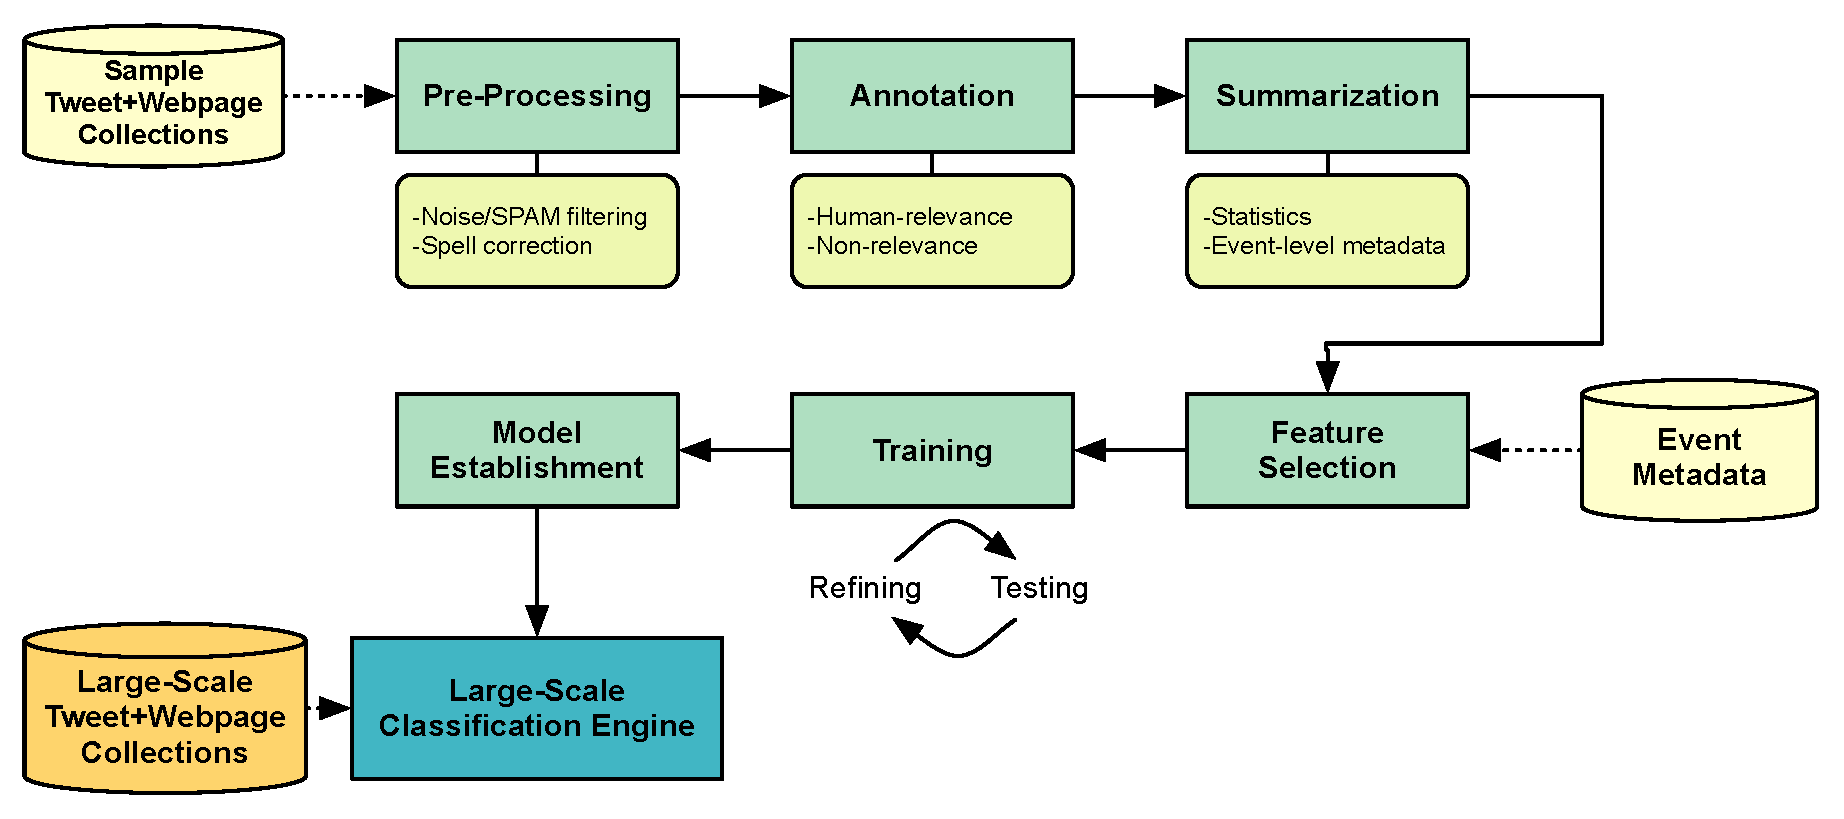
\includegraphics[width=0.9\textwidth]{figs/classification-pipeline.eps}
 \caption{\small Classification pipeline.  \label{fig:pipeline}}
\end{figure}

\begin{table}[t]
\centering
 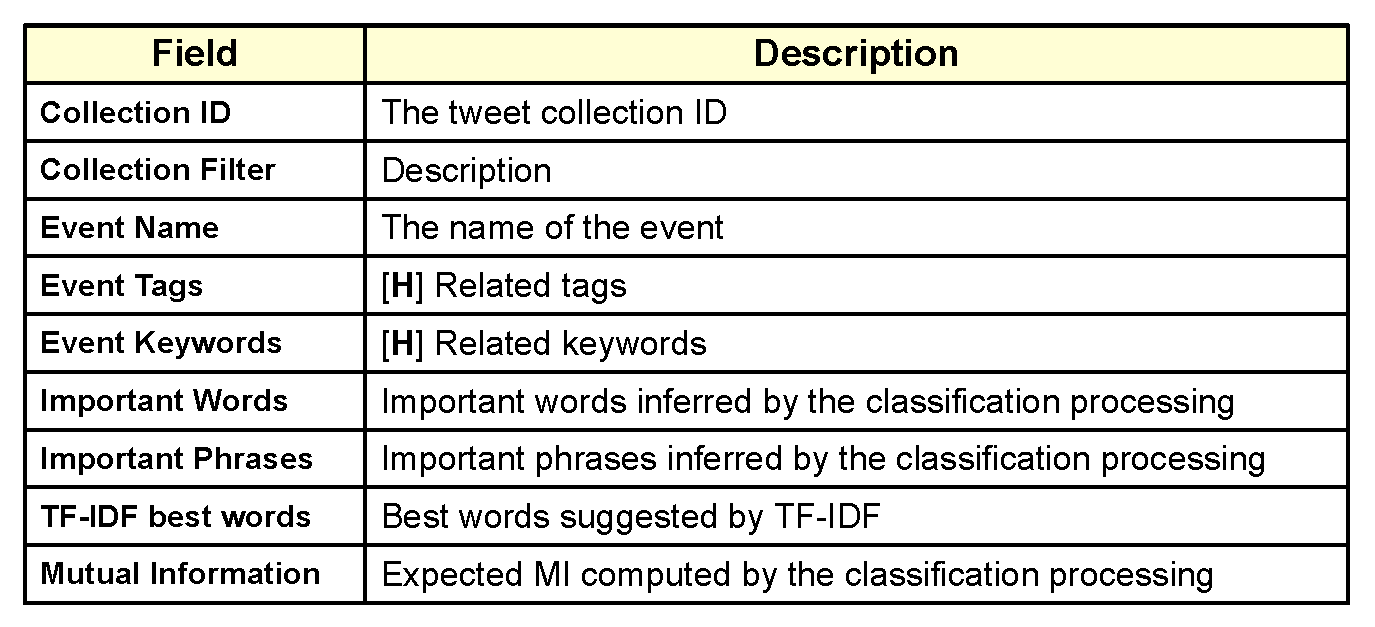
\includegraphics[width=0.8\textwidth]{figs/classmetadata.eps}
 \caption{\small Classification metadata. \label{tbl:metadata}}
\end{table}

\begin{figure}[t]
\centering
 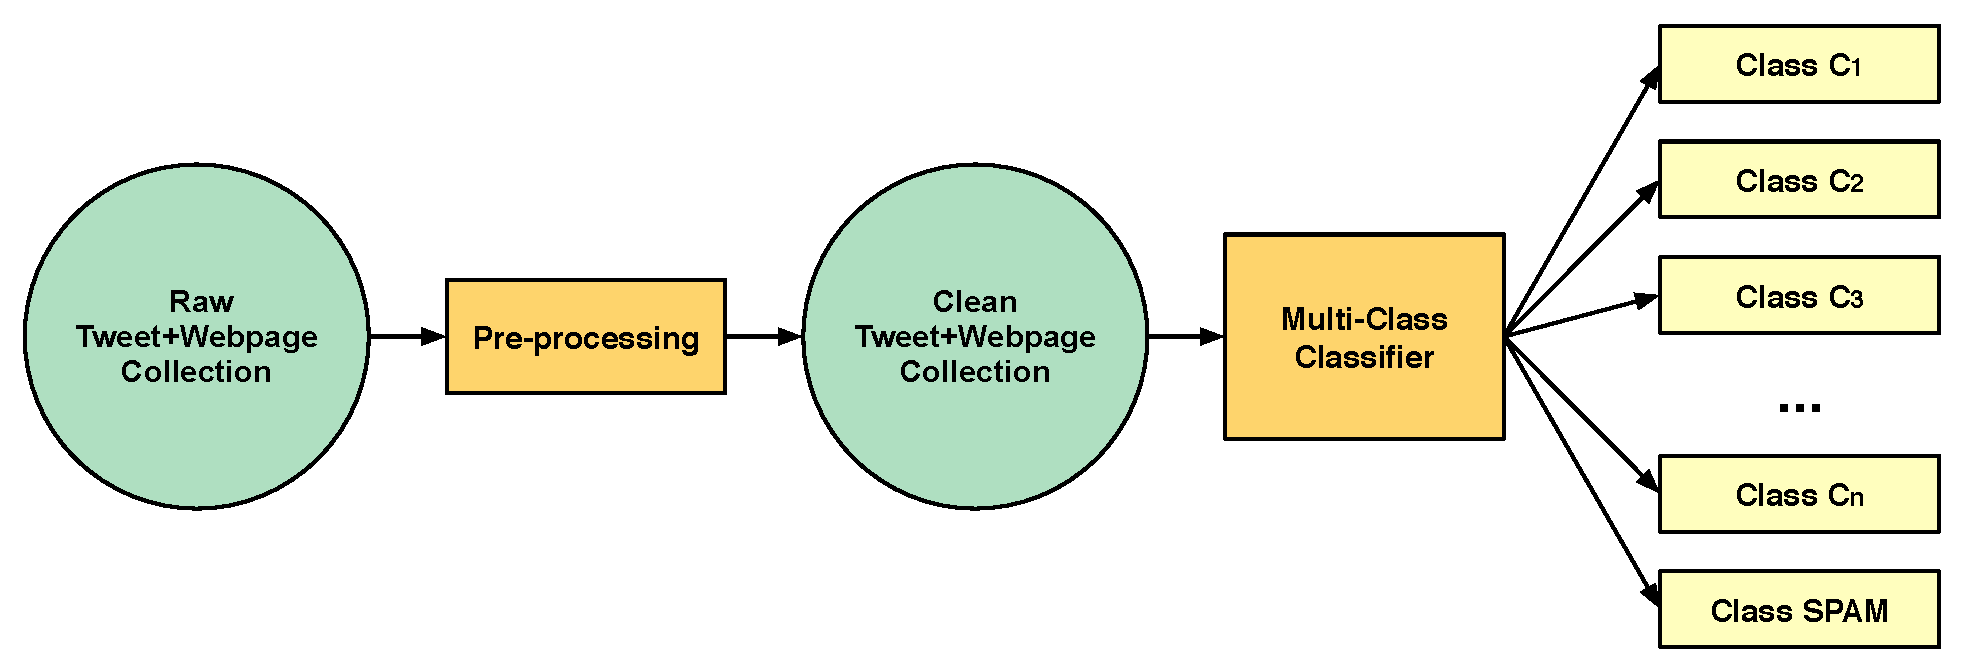
\includegraphics[width=0.9\textwidth]{figs/trainingapproach.eps}
 \caption{\small Training data approach. \label{fig:trainingapproach}}
\end{figure}


